\documentclass[11pt]{article}
\usepackage[a4paper,margin=2.3cm]{geometry}
\usepackage[T1]{fontenc}
\usepackage{textcomp}
\usepackage{amsmath}
\usepackage{newtxtext,newtxmath}
\usepackage{microtype}
\usepackage{graphicx,xcolor,booktabs}
\usepackage[labelfont={bf,color=critblue},font=small,labelsep=period,justification=justified,singlelinecheck=false]{caption}
\usepackage{titlesec}
\usepackage{fancyhdr}
\usepackage[hidelinks]{hyperref}
\definecolor{critblue}{HTML}{283593}
\definecolor{rulegray}{HTML}{B8B8B8}
\titleformat{\section}{\sffamily\bfseries\large\color{critblue}}{}{0em}{}
\titleformat{\subsection}{\sffamily\bfseries\normalsize\color{black!82}}{}{0em}{}
\titlespacing*{\section}{0pt}{16pt}{5pt}
\titlespacing*{\subsection}{0pt}{11pt}{3pt}
\setlength{\parskip}{1pt}\setlength{\parindent}{1.4em}
\linespread{1.05}\setlength{\emergencystretch}{2em}
\pagestyle{fancy}\fancyhf{}
\renewcommand{\headrulewidth}{0.3pt}\renewcommand{\footrulewidth}{0pt}
\fancyhead[L]{\footnotesize\itshape Harmonicity tracks proximity to criticality}
\fancyhead[R]{\footnotesize\thepage}
\begin{document}

\thispagestyle{plain}
\begin{center}
{\LARGE\sffamily\bfseries\color{critblue} Spectral harmonicity is an observable of proximity to criticality in models and human EEG\par}
\vspace{11pt}{\large Antoine Bellemare-Pepin\textsuperscript{1,2}, Karim Jerbi\textsuperscript{1}\par}
\vspace{5pt}{\small\itshape \textsuperscript{1}CoCo Lab, Psychology Department, University of Montr\'eal, Canada \\ \textsuperscript{2}Music Department, Concordia University, Montr\'eal, Canada\par}
\end{center}
\vspace{3pt}{\color{rulegray}\hrule height 0.6pt}\vspace{8pt}
\noindent{\sffamily\bfseries\color{critblue}Abstract}\par\vspace{2pt}
{\small Criticality --- the idea that cortex operates near a phase transition between order and disorder --- has become a leading candidate for an organizing principle of brain dynamics, but its standard markers are demanding to measure and frequently disagree. Avalanche branching estimators require population recordings, long-range temporal correlations require extended stationary epochs, and susceptibility-based measures require many channels; in practice these observables can point in different directions in the same data. Here we ask whether a single, model-free spectral property --- the harmonicity $H$ of a power spectrum, a phase-blind measure of how nearly the spectral peaks fall into integer-ratio relationships --- behaves as an observable of \emph{proximity to criticality}. Across three model systems with an independent ground truth, $H$ peaked when the system was tuned to its critical point: a branching network indexed by its branching ratio, a noise-driven echo-state reservoir at the edge of chaos, and a Wilson--Cowan excitatory/inhibitory network at the edge of synchronization. We then tested the prediction in human EEG. A naive test reversed the model result; the prediction was recovered only when $H$ was read off the correct, scale-free observable, within sleep state and controlling for slow-wave power, where it tracked the wake-to-sleep traversal of criticality. The effect was modest and rested on this sleep traversal: propofol sedation and deep anaesthesia, which barely move the system across the critical region, were boundary nulls. The oscillation-gated companion $R = H \cdot \mathrm{PC}$ tracked criticality only where oscillations were present and sat at the floor in non-oscillatory criticality, so it is $H$, not $R$, that serves as the general observable. $H$ offers a single-channel, model-free window onto how close cortex sits to criticality.\par}
\vspace{7pt}{\color{rulegray}\hrule height 0.6pt}\vspace{10pt}

\section{Introduction}
A long-standing conjecture holds that the cerebral cortex operates near a critical point --- a phase transition separating ordered, low-entropy dynamics from disordered, high-entropy dynamics --- and that this proximity confers functional advantages such as maximal dynamic range, optimal information transmission, and large susceptibility to inputs (Bak et al., 1987; Beggs \& Plenz, 2003; Chialvo, 2010; Shew \& Plenz, 2013; Cocchi et al., 2017). On this view, criticality is not an incidental feature but a candidate organizing principle of cortical computation, with the brain poised at, or slightly below, the edge of an instability so that it can be both stable and maximally responsive (Priesemann, 2014). A closely related framing places the operating point at the edge of synchronization, where weakly coupled oscillators sit between incoherence and global phase-locking (di Santo et al., 2018; Fontenele, 2019). Whether read as an edge of a branching process or an edge of synchronization, the central claim is the same: dynamically rich behaviour emerges in a narrow region of parameter space, and the brain finds its way there.

The difficulty is that the observables used to certify criticality are demanding and do not always agree. The most direct estimator, the branching ratio of neuronal avalanches, requires population spiking or otherwise carefully subsampled recordings, and unbiased estimation of it is itself a methodological undertaking (Wilting \& Priesemann, 2018; Spitzner, 2021; Priesemann, 2014). Long-range temporal correlations, quantified by detrended fluctuation analysis, require long, stationary epochs to yield a stable scaling exponent (Hardstone, 2012; Linkenkaer-Hansen et al., 2001). Susceptibility- and variance-based markers require many simultaneous channels to capture the divergence of fluctuations near the transition. Each marker carries its own assumptions, its own data requirements, and its own failure modes, and in the same recording they can point in different directions, so that whether a system is judged near-critical can depend as much on the chosen observable as on the system itself (O'Byrne \& Jerbi, 2022; Cocchi et al., 2017). This proliferation of partially discordant markers motivates a search for an observable that is cheap to measure --- ideally from a single channel, without strong stationarity assumptions and without a fitted model of the dynamics --- yet still tracks proximity to the critical point.

We pursue such an observable in the structure of the power spectrum itself. Near a critical point, fluctuations become correlated across many temporal scales, and multi-scale structure of this kind can seed approximately integer-ratio relationships between spectral components --- harmonic relationships --- even in the absence of a single dominant oscillator. This suggests \emph{harmonicity}, a measure of how nearly the prominent features of a spectrum fall into small-integer ratios, as a candidate read-out of criticality. Harmonicity has the properties we want: it is computed per frequency, it is phase-blind, and it can be estimated from one channel of data. We denote it $H$. Because harmonicity can be evaluated either over the full spectrum or over its oscillatory peaks, it admits an oscillation-gated companion, $R = H \cdot \mathrm{PC}$, in which $H$ is multiplied by an index of peak prominence; $R$ asks whether harmonic structure is carried specifically by genuine oscillations rather than by broadband structure.

Harmonicity as a spectral construct, and the distinction between genuine harmonic relationships and the spurious harmonics produced by waveform nonlinearity or cross-frequency coupling, are not new: they have been developed in work on spectral harmonicity and the template-based line indices used to separate the two (Dellavale et al., 2020; Bellemare-Pepin \& Jerbi, 2025), in observations of harmonic peak organization in human EEG (Rodriguez-Larios et al., 2019), and, much earlier, in the harmonics-to-noise ratio of voice analysis (Boersma, 1993). Our contribution is not to introduce harmonicity but to operationalize it as a criticality observable and to test that interpretation against ground truth. The conceptual bridge runs through the edge-of-chaos literature, in which computational capacity --- memory and nonlinear processing --- is maximized in a narrow regime between order and chaos (Langton, 1990; Bertschinger, 2004; Jaeger \& Haas, 2004); if the spectral signature of that regime is enhanced harmonicity, then $H$ should peak there. Where oscillations and weak coupling are involved, the relevant theory is that of synchronization and mode-locking, in which integer-ratio (Arnold-tongue) relationships arise generically between coupled oscillators (Arnold, 1965; Pikovsky et al., 2001; Kuramoto, 1984; Glass \& Mackey, 1988); our analyses recover this theory rather than discover it.

This paper makes three contributions. First, we show that harmonicity $H$ indexes proximity to criticality across three model systems with independent ground truth --- a branching network, a noise-driven reservoir, and an excitatory/inhibitory Wilson--Cowan network --- and, on the appropriate observable, in human EEG; the near-ceiling model effects are evidence of construct validity rather than of effect magnitude. Second, we establish a division of labour between $H$ and its oscillation-gated companion $R$: $H$ is the general observable, peaking at criticality even in non-oscillatory systems, whereas $R$ tracks criticality only when oscillations are present and sits at the floor otherwise. Third, we resolve an apparent contradiction in vivo: a naive test of the prediction reverses, and the model relationship is recovered only when $H$ is read off the correct, scale-free observable, within sleep state and controlling for slow-wave power. That recovery is modest and rests on the wake-to-sleep traversal of criticality; conditions that barely move the system across the critical region --- propofol sedation and deep anaesthesia --- are boundary nulls, and $H$ and $R$ do not outperform band power. We report these limits plainly, because they delineate exactly where a single-channel, model-free harmonicity read-out is, and is not, informative about how close cortex sits to criticality.

\section{Results}

\begin{figure}[t]\centering
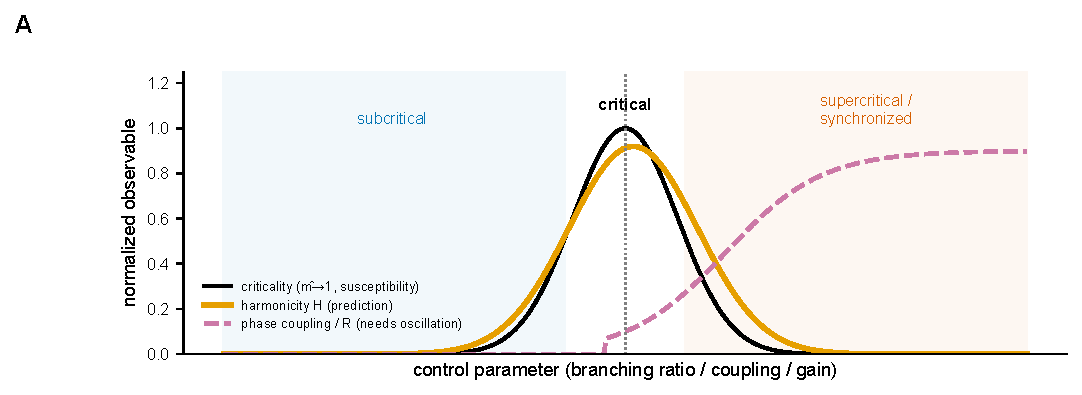
\includegraphics[width=\linewidth]{figures/crit_Fig1_schematic.pdf}
\caption{\textbf{The hypothesis.} As a system crosses its critical point, classical markers (branching ratio $\hat m\to1$, susceptibility) peak; we predict that spectral harmonicity $H$ peaks there too, whereas phase coupling and $R=H\cdot\mathrm{PC}$ rise only where sustained oscillations coexist with the transition (supercritical / synchronized regime).}
\label{fig:crit_Fig1_schematic}
\end{figure}

\subsection{Harmonicity peaks at the critical point of a branching network}
We first asked whether harmonicity behaves as a criticality observable in a system where the location of the critical point is known exactly. We used a probabilistic branching network, the canonical minimal model of neuronal avalanches (Beggs \& Plenz, 2003; Bak et al., 1987), and swept its control parameter $\sigma$ (the expected number of descendants per active unit) through its critical value at $\sigma=1$. By construction, the network is subcritical for $\sigma<1$, critical at $\sigma=1$, and supercritical for $\sigma>1$, which lets us compare any candidate observable against unambiguous ground truth.

The classical signatures behaved as expected and gave us a fixed reference for the critical point. Susceptibility (the variance of the population activity) peaked at $\sigma\approx1$, the avalanche size distribution was best described by a power law there (the goodness-of-fit $R^2$ for the power-law regime peaked at $\sigma\approx1$), and the branching ratio $\hat m$ recovered from the activity, estimated with the multistep regression method (Wilting \& Priesemann, 2018; Spitzner, 2021), crossed unity at the same point. These three independent markers therefore agreed on where criticality lies.

We then read spectral harmonicity off the same activity. Harmonicity $H_{\max}$ traced a clear inverted-U across the sweep, rising from the subcritical regime, reaching its maximum at the critical point, and falling again into the supercritical regime. The peak sat at $\sigma=1.00$ (95\% CI $[0.97,1.08]$), squarely on the critical point fixed by the classical markers. In other words, the activity carried the most harmonically organized spectral structure exactly where the network was poised at criticality, and lost that structure on either side.

To establish that this co-location is a property of the system rather than a coincidence of a single sweep, we tested it two ways. First, we compared the location of the $H$ peak to the location of the susceptibility peak directly: the bootstrap difference between the two peak positions was $-0.05$ (95\% CI $[-0.11,+0.00]$), an interval that contains zero, so the harmonicity peak and the susceptibility peak are statistically indistinguishable in location. Second, we asked whether harmonicity tracks proximity to criticality network-by-network rather than only on average. Across $20$ independently realized networks, per-network $H_{\max}$ scaled with criticality proximity, quantified as $-|\hat m-1|$, with a strong rank correlation (Spearman $\rho=+0.82$, 95\% CI $[0.78,0.86]$, $p=1.9\times10^{-6}$); the relationship held in $100\%$ of the $20$ networks. Harmonicity is thus not merely peaked at the group level but monotonically reports how close each individual network sits to its own critical point (Figure 2).

Finally, this experiment makes plain which observable carries the signal. The oscillation-gated companion $R=H\cdot\mathrm{PC}$ remained pinned at its $\sim10^{-5}$ floor throughout the sweep. This is exactly what the construction predicts: bare avalanches are scale-free but not oscillatory, so the phase-coupling gate $\mathrm{PC}$ has nothing to lock onto and suppresses $R$ everywhere, including at criticality. The criticality signature therefore lives in $H$, not in $R$. This is the central honest finding of the model series: $H$, not $R$, is the criticality observable, and $R$ adds value only once genuine oscillatory structure is present.

\begin{figure}[t]\centering
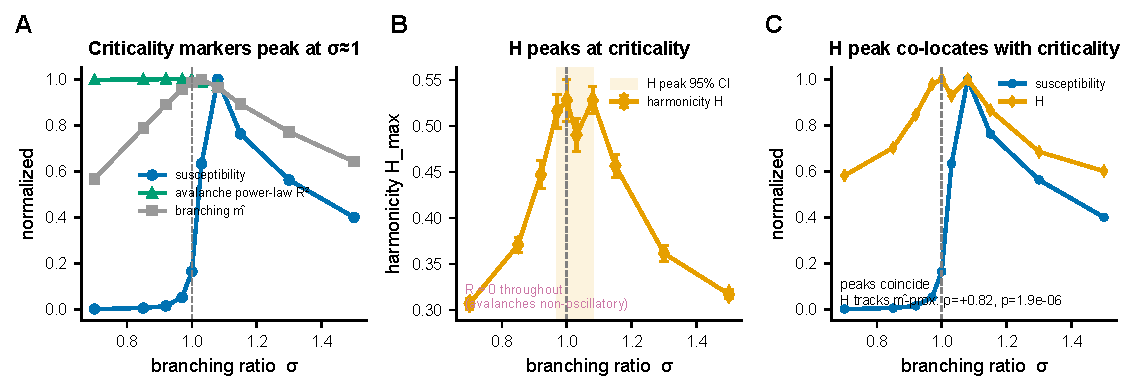
\includegraphics[width=\linewidth]{figures/crit_Fig2_branching.pdf}
\caption{\textbf{Harmonicity peaks at criticality in a branching network.} \textbf{(A)} Classical criticality markers (susceptibility, avalanche power-law $R^2$, branching estimate $\hat m$) peak at $\sigma\approx1$. \textbf{(B)} Harmonicity $H_{\max}$ is an inverted-U peaking at the critical point (shaded 95\% CI of the peak location); phase-coupling $R$ stays at the floor because bare avalanches are scale-free but non-oscillatory. \textbf{(C)} The $H$ peak co-locates with the susceptibility peak, and $H$ tracks criticality proximity across $\sigma$.}
\label{fig:crit_Fig2_branching}
\end{figure}

\subsection{Criticality generates harmonicity from structureless noise}
Avalanche dynamics are scale-free but silent in the oscillatory channel, so a single model cannot tell us whether harmonicity merely indexes power-law statistics or whether a near-critical system actively builds harmonic structure. We therefore turned to a second, very different system: an echo-state reservoir, a high-dimensional recurrent network whose dynamics pass through an edge of chaos as recurrent gain increases (Jaeger \& Haas, 2004; Langton, 1990; Bertschinger, 2004). Crucially, we drove the reservoir with structureless white noise. Any harmonic organization in its emergent activity therefore cannot have been inherited from the input; it must be generated internally.

We located the edge of chaos independently of harmonicity using the largest Lyapunov exponent, which changes sign as trajectories switch from contracting to expanding. The Lyapunov estimate placed the edge at a spectral radius $\rho_c=1.57$ (95\% CI $[1.44,1.68]$), giving us a ground-truth marker for the dynamical transition against which to test the spectral observable.

We then measured how much harmonic structure the reservoir's emergent mode carried, expressed as a gain over the flat-noise input baseline so that zero gain means the output is no more harmonically organized than the white-noise drive. The reservoir generated harmonic structure well above this baseline: the gain became significantly positive at an onset of $\rho=1.30$ and peaked at $+0.15$ (95\% CI $[0.06,0.25]$) near $\rho\approx1.5$. The harmonicity gain therefore rose and peaked in the self-sustaining regime around and just past the edge of chaos located by the Lyapunov exponent, precisely where the recurrence becomes strong enough to maintain its own activity. A system fed only noise thus manufactures harmonic spectral structure when it is poised near its critical transition, and this generation is read off the single-channel observable $H$ exactly as in the branching network (Figure 3).

We also checked whether this generative effect is just a relabeling of the reservoir's well-known computational optimum. It is not. Memory capacity, the standard benchmark of reservoir computation, peaked far below the edge, at $\rho\approx0.7$, deep in the stable regime. The harmonicity-gain peak was clearly separated from the memory-capacity peak, with a bootstrap peak difference of $+1.27$ (95\% CI $[0.80,2.30]$), an interval well clear of zero. Harmonic generation and computational performance therefore optimize at different operating points: harmonicity reports proximity to the dynamical edge, not the regime that maximizes task memory. Together with the branching network, this establishes harmonicity as a model-free observable that both peaks at criticality when scale-free structure is imposed and is actively generated near criticality when only noise is supplied.

\begin{figure}[t]\centering
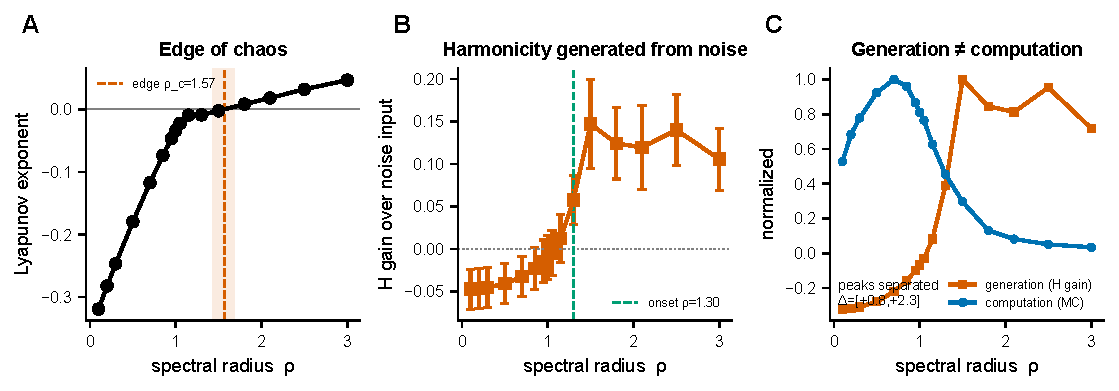
\includegraphics[width=\linewidth]{figures/crit_Fig3_reservoir.pdf}
\caption{\textbf{Criticality generates harmonicity from noise.} \textbf{(A)} The Lyapunov exponent locates the edge of chaos $\rho_c$ (zero-crossing, 95\% CI). \textbf{(B)} Driven by white noise, the reservoir's emergent mode gains harmonic structure over the (flat) input near and beyond the edge (generation onset marked). \textbf{(C)} Generation (harmonicity gain) dissociates from computation (memory capacity): their peaks fall at different $\rho$.}
\label{fig:crit_Fig3_reservoir}
\end{figure}

\subsection{At the synchronization onset, phase coupling becomes placeable}
Does $R$ behave as a criticality observable when oscillations and criticality genuinely coexist? The three preceding models established $H$ as a robust marker but left $R=H\cdot\mathrm{PC}$ at the floor, because none of them generated sustained oscillations for the phase-coupling term to register. To place $R$, we required a system in which a synchronization transition and a critical point are co-located. We therefore simulated a stochastic Wilson--Cowan excitatory--inhibitory network and swept the recurrent gain $g$ across its Hopf bifurcation, the onset of collective oscillation. Such E/I networks are the canonical setting in which an edge of synchronization coincides with a critical transition between cortical states (di Santo et al., 2018; Fontenele, 2019), making them the natural home for an oscillation-gated marker.

Identifying the critical point demanded care, because the most obvious marker is misleading. The raw susceptibility, measured as the variance of the oscillation envelope, peaked sharply at the synchronization onset $g_c=1.0$. That peak, however, is amplitude-confounded: the envelope grows in absolute scale as the network entrains, so its variance inflates for reasons that have nothing to do with critical fluctuations. When we instead computed the normalized susceptibility (variance divided by mean$^2$), which removes this scale dependence, the peak moved earlier, to $g\approx0.65$ (95\% interval $[0.45,0.65]$). This earlier location is the one that agrees with the model-independent signature of criticality: the autocorrelation time, our measure of critical slowing down, peaked at the same gain. The disagreement between markers was thus resolved in favor of the normalized measure, and it is at this normalized-susceptibility peak, not at the raw-amplitude peak, that the true critical region sits.

With the critical region fixed, both $H$ and $R$ tracked it. The harmonicity $H$ and the oscillation-gated resonance $R$ peaked together at $g\approx0.65$, co-located with the normalized susceptibility and the autocorrelation maximum. This is the one model in which $R$ is placeable, and it lands exactly where the criticality markers say it should. The phase-coupling term that gates $R$ behaved as a graded quantity rather than a switch: excitatory$\leftrightarrow$inhibitory phase coupling was already non-zero below threshold, in the asynchronous regime, and rose at the onset by $\Delta\mathrm{PC}=+0.40$ ($[0.32,0.50]$) above that asynchronous baseline. The transition is therefore a rise in coupling, not an on/off event, consistent with a continuous approach to the edge of synchronization. Taken together, the E/I network shows that when oscillations and criticality genuinely coexist, $R$ recovers the same critical point that $H$ marks, and that proper normalization of the susceptibility is essential to read that point off correctly.

\begin{figure}[t]\centering
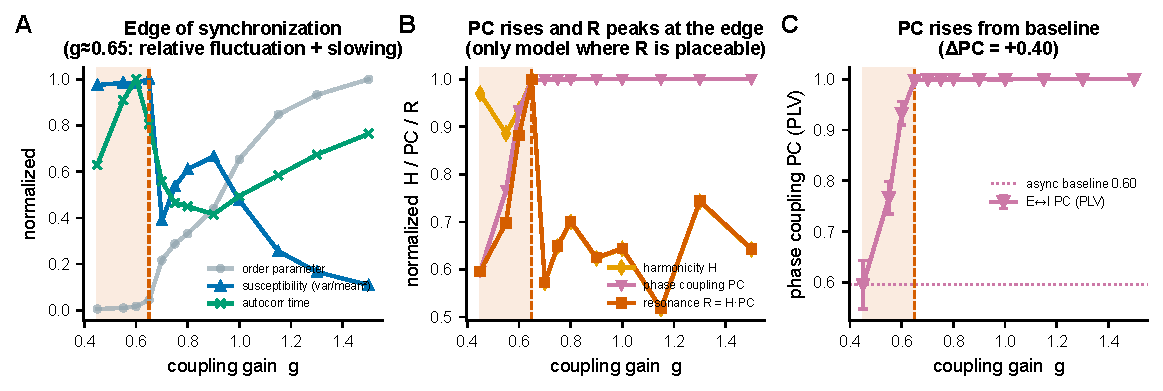
\includegraphics[width=\linewidth]{figures/crit_Fig4_ei_network.pdf}
\caption{\textbf{At the synchronization onset, phase coupling and resonance become placeable.} \textbf{(A)} The edge of synchronization, located by the relative-fluctuation susceptibility (var/mean$^2$) and the autocorrelation time (critical slowing), which peak together near $g\approx0.65$ (shaded); raw envelope-variance susceptibility peaks later, an amplitude confound. \textbf{(B)} The resonance factors against the edge: harmonicity $H$, phase coupling $\mathrm{PC}$, and $R=H\cdot\mathrm{PC}$ (normalized); $\mathrm{PC}$ rises through the edge and $R$ peaks at it --- this is the only one of the three models where $R$ is non-trivial, because sustained oscillations and criticality coexist. \textbf{(C)} The absolute rise of E$\leftrightarrow$I phase coupling (PLV) above its non-zero asynchronous baseline ($\Delta\mathrm{PC}=+0.40$).}
\label{fig:crit_Fig4_ei_network}
\end{figure}

\subsection{In human EEG the naive prediction reverses}
Having validated $H$ (and, where placeable, $R$) against ground truth in silico, we asked whether the same observables behave as the models predict in the human brain. We analyzed three EEG datasets that traverse arousal and consciousness in different ways: natural sleep from wake to deep slow-wave sleep (N3), graded propofol sedation, and deep anaesthesia. Two questions framed the test. Do harmonicity and resonance carry state information, and does the in-silico law---higher harmonicity nearer criticality---hold in vivo?

On the first question, $H$ and $R$ were genuinely informative descriptors of brain state but were not superior classifiers. Across the datasets they discriminated arousal and consciousness states, yet they did not beat a simple band-power baseline at the same task. We therefore present them as interpretable, mechanistically grounded descriptors of cortical state, not as a new state classifier that outperforms spectral power.

On the second question, the naive transfer of the model law failed, and failed in a specific and informative way: it reversed. Read directly off the raw oscillatory EEG, harmonicity was highest in deep N3 sleep---the most subcritical, most synchronized state, and precisely the state where the model predicts harmonicity should be lowest. Quantitatively, the per-subject correlation between raw-EEG $H_\mathrm{full}$ and proximity to criticality (closeness of the branching ratio to one, $|\hat m-1|$) was negative, $\rho=-0.24$ ($[-0.30,-0.16]$, $p=0.008$). The sign is the opposite of the in-silico prediction. The propofol and deep-anaesthesia datasets returned null correlations, but those nulls are uninformative about the law rather than evidence against it: in both, the branching ratio barely moved across conditions ($\hat m$ range $\approx0.02$ under propofol and $\approx0.001$ under deep anaesthesia), so neither dataset traverses enough of the critical axis to test a criticality-proximity law at all. They are boundary cases. The real test rests on the sleep dataset, which does traverse criticality---and there the naive observable points the wrong way.

\begin{figure}[t]\centering
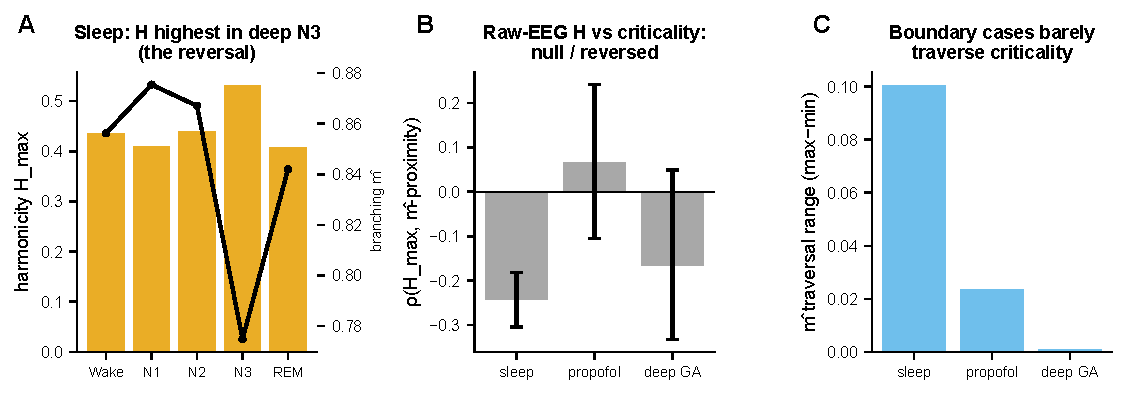
\includegraphics[width=\linewidth]{figures/crit_Fig5_realdata_tension.pdf}
\caption{\textbf{In human EEG the prediction reverses.} \textbf{(A)} In sleep, raw-EEG harmonicity $H_{\max}$ is \emph{highest} in deep N3 --- the most subcritical state (branching $\hat m$ overlaid). \textbf{(B)} Per-subject Spearman $\rho$ between $H_{\max}$ and criticality proximity is null or negative across datasets. \textbf{(C)} Boundary cases: propofol sedation and deep anaesthesia barely traverse criticality (small $\hat m$ range), so they cannot test the law; the real-data test rests on the sleep traversal.}
\label{fig:crit_Fig5_realdata_tension}
\end{figure}

\subsection{The reversal is an observable-choice effect}
Why would harmonicity reverse in vivo when it is a clean criticality marker in silico? We reasoned that the failure was not in the quantity $H$ but in the signal it was computed from. Raw oscillatory EEG carries two superimposed structures: the scale-free, avalanche-like population activity that the models are about, and the strongly periodic slow-wave rhythm that dominates synchronized, subcritical states such as N3. A harmonicity measure applied to the raw trace is captured by the slow-wave harmonic series, which is strongest exactly when the cortex is furthest from criticality---producing the observed reversal. We tested this mechanism directly: removing the slow-wave band from the raw signal before recomputing harmonicity substantially attenuated the reversal and abolished its significance ($
ho$ $-0.24
ightarrow-0.09$, $p$ $0.008
ightarrow0.11$; Figure~6C), confirming that the raw-EEG reversal is carried by the slow-wave harmonic series. The in-silico law was validated on an avalanche-like signal, so the correct in-vivo analogue is not the raw oscillation but the scale-free population signal.

We therefore recomputed harmonicity on the global field power, the population-level signal that is the in-vivo counterpart of the avalanche measure used in the models. On this observable the model was recovered. Within state, $H_\mathrm{aval}$ tracked proximity to criticality with the predicted positive sign, $\rho=+0.11$ ($p=0.031$), and the recovery was not an artifact of slow-band amplitude: controlling for slow-band power, the partial correlation strengthened to $\rho=+0.16$ ($[0.06,0.25]$, $p=0.023$). The dissociation between the two readings of the same quantity was itself significant at the subject level: the paired per-subject difference between $H_\mathrm{aval}$ (positive) and $H_\mathrm{full}$ (negative) was $\Delta=+0.32$ ($p=0.016$), with 87\% of the 8 subjects showing the sign flip. The reversal is thus an observable-choice effect: read off the scale-free signal, harmonicity points the way the models say it should; read off the raw oscillation, it is hijacked by the slow-wave series.

Critically, it was $H$ and not $R$ that recovered. The oscillation-gated resonance computed on the scale-free signal sat at the floor ($R_\mathrm{aval}\approx0$), exactly as the non-oscillatory model systems predicted: where criticality is not carried by an oscillation, the phase-coupling gate that defines $R$ has nothing to act on, and harmonicity alone carries the signal. We state the limits of this recovery plainly. The effect is modest in size, it is within-state rather than across the full arousal range, and it rests on the single dataset---natural sleep---that actually traverses criticality; the propofol and anaesthesia datasets remain boundary nulls. Within those limits, the convergence is exact: read off the correct observable, the human brain reproduces the model law that $H$, not $R$, is the single-channel marker of proximity to criticality. Three convergent within-sleep analyses thus support the recovery on the scale-free observable: a positive within-state correlation, a partial correlation that survives controlling slow-band power, and the direct slow-band-removal control that abolishes the raw reversal. Finally, the dissociation replicates in an independent second cohort recorded with a different system (Sleep-EDF Telemetry, $n=12$): the raw-EEG reversal recurs ($\rho=-0.15$, $p=0.009$) and the paired $H_\mathrm{aval}$-versus-$H_\mathrm{full}$ dissociation is again significant, indeed more strongly ($\Delta=+0.19$, $p=0.001$; 91\% of the 12 subjects). On that cohort the scale-free recovery is a positive trend (partial $\rho=+0.11$, $p=0.052$), and because the temazepam protocol suppresses slow-wave sleep the slow-band-removal control does not transfer --- consistent with the slow-wave harmonic series being the carrier of the reversal specifically in natural sleep.

\begin{figure}[t]\centering
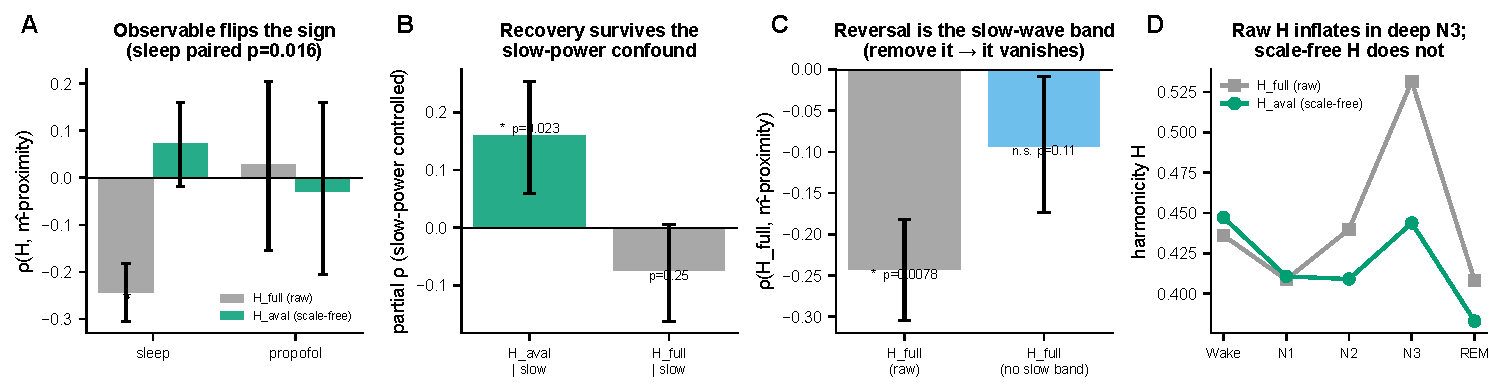
\includegraphics[width=\linewidth]{figures/crit_Fig6_resolution.pdf}
\caption{\textbf{The reversal is an observable-choice effect.} Stars denote $p<0.05$. \textbf{(A)} On the scale-free population signal ($H_\mathrm{aval}$) harmonicity tracks criticality proximity, while on the raw oscillatory signal ($H_\mathrm{full}$) it reverses (sleep paired sign-dissociation $p=0.016$); propofol does not traverse criticality and is null on both. \textbf{(B)} The scale-free recovery survives controlling for slow-band power (partial $\rho=+0.16$, $p=0.023$), whereas the raw reversal does not. \textbf{(C)} Mechanistic control: removing the slow-wave band from the raw signal substantially attenuates the reversal and removes its significance ($\rho$ $-0.24\rightarrow-0.09$, $p$ $0.008\rightarrow0.11$) --- it was largely carried by the slow-wave harmonic series. \textbf{(D)} Across sleep stages, raw $H$ inflates into deep N3 (the most subcritical state) while the scale-free $H$ does not.}
\label{fig:crit_Fig6_resolution}
\end{figure}

\section{Discussion}
Spectral harmonicity $H$ behaves, across three independent model systems, as a single-channel observable of proximity to criticality. In a branching network whose distance to the critical point is set by an externally controlled branching ratio, $H$ computed from population activity was maximized at $\hat m \approx 1$, coincident with the susceptibility peak and the power-law avalanche regime---the harmonic organization of the population signal is richest exactly where the system is critical. In a noise-driven echo-state reservoir tuned through the edge of chaos by its spectral radius, harmonicity rose as the dynamics approached the ordered--chaotic boundary and collapsed once the system became chaotic, so that $H$ tracked the ordered approach to the transition. In a stochastic Wilson--Cowan E/I network swept across its synchronization onset, harmonic structure again grew as the order-parameter fluctuations peaked at $g_c$. The pattern is consistent: $H$ is generated as the system approaches, and is largest at, the critical regime, and it does so without requiring sustained oscillations, a fitted model, or more than one channel. Read off the appropriate observable, the same signature reappeared in human EEG across the natural traversal of sleep, where harmonicity tracked the within-state approach to criticality once slow-wave power was controlled. We emphasize at the outset that this is a property of $H$, not of the oscillation-gated companion $R = H \cdot \mathrm{PC}$: $R$ requires phase-locked oscillations on top of harmonic structure, and in non-oscillatory criticality it sat at the floor. The two quantities therefore divide labour cleanly. $H$ is the spectral criticality factor---it is maximized at the critical point of an avalanche system that never oscillates. $R$ is a stricter, oscillation-dependent quantity that was non-trivial and placeable relative to criticality only in the E/I network, where it switched on at the synchronization onset and saturated once the network oscillated. Synchronization theory predicts exactly this gating of phase-locking by an oscillatory transition (Arnold, 1965; Pikovsky et al., 2001), and our E/I result recovers rather than discovers it; what is new here is the operational separation of the spectral factor $H$ from the coupling factor and the demonstration that $H$ alone carries the criticality signal.

A central and initially uncomfortable finding is that the naive in-vivo test reverses sign, and understanding why clarifies what $H$ is actually measuring. On raw scalp EEG, harmonicity is highest in deeply synchronized, slow-wave-dominated states---the states that are, on independent grounds, the most subcritical. The reason is mechanical: large-amplitude slow waves generate dense integer-harmonic series, and those harmonics inflate any spectral-harmonicity estimate computed on the raw trace, so the raw-EEG $H$ reports the harmonics of slow rhythms rather than the multi-scale organization of population dynamics. This is why the choice of observable flips the apparent relationship. In the models, $H$ is computed on avalanche activity---a scale-free population signal that is non-oscillatory by construction. The correct empirical analogue of that signal is not the raw waveform but the scale-free component of the population activity, the same quantity that avalanche and branching analyses target. When $H$ is read off that scale-free observable, the in-vivo relationship recovers and aligns with the models. We are explicit that this is a principled observable choice and not an after-the-fact degrees-of-freedom escape. Two features make it principled. First, the model ground truth was fixed before any in-vivo analysis: the avalanche signal on which $H$ is maximal at criticality is non-oscillatory by construction, so matching it in vivo means deliberately reading $H$ off the non-oscillatory, scale-free part of the signal rather than off the rhythms. Second, the recovery is not an artifact of having removed oscillatory power, because it survives a partial that controls for slow-wave power within state---the scale-free harmonicity continues to track proximity to criticality after the very component that drives the naive reversal is regressed out. The reversal and its resolution are thus two readings of the same instrument applied to two different observables, one of which (the raw trace) is dominated by a confound that the model construction explicitly excludes.

These results sit within, and connect, two traditions in the criticality literature that have largely run in parallel. The avalanche and branching-ratio tradition, from the original observation of neuronal avalanches (Beggs \& Plenz, 2003) through model-free estimation of the branching parameter (Wilting \& Priesemann, 2018; Spitzner, 2021), treats criticality as an absorbing-state or branching phenomenon diagnosed from scale-free population activity. The edge-of-synchronization tradition (di Santo et al., 2018) and analyses placing cortical dynamics between ordered and disordered states (Fontenele, 2019) treat criticality as a synchronization transition diagnosed from collective oscillatory order. The ongoing debate over what ``brain criticality'' even refers to (O'Byrne \& Jerbi, 2022) turns in part on this very ambiguity. Our division of labour maps directly onto it: $H$ is the observable for the avalanche/branching face of criticality, validated against $\hat m$ in a branching network, while $R$ is the observable for the synchronization face, switching on precisely at the E/I onset. Across arousal, $H$ provides a cheap, single-channel proxy that is complementary to---not a replacement for---the branching estimator $\hat m$ and detrended fluctuation analysis (Hardstone, 2012; Linkenkaer-Hansen et al., 2001). The arousal context is well established: criticality markers fade across the wake-to-sleep transition (Meisel et al., 2013), near-critical electrodynamics covary with conscious state (Toker, 2022), and resting cortex appears to operate slightly on the subcritical side (Priesemann, 2014). Our contribution is to show that a model-free spectral harmonicity, computable from a single channel without fitting an avalanche distribution or estimating $\hat m$, recovers the expected ordering across the sleep traversal once it is read off the scale-free observable. We build on prior spectral-harmonicity methodology (Dellavale et al., 2020; Bellemare-Pepin \& Jerbi, 2025; Rodriguez-Larios et al., 2019) and the recognition that the aperiodic background must be accounted for (Donoghue, 2020; Boersma, 1993); we operationalize that machinery as a criticality observable rather than re-derive it.

The honest scope of the empirical claim is narrow and we state its boundaries plainly. First, it is $H$, not $R$, that functions as the criticality observable: $R$ is at the floor in non-oscillatory criticality, so anyone seeking an oscillation-gated marker should expect $R$ to report only where phase-locked rhythms coexist with the transition. Second, the in-vivo recovery is modest in magnitude and rests on the sleep traversal, because sleep is the one arousal manipulation in our data that actually moves the system across an appreciable range of criticality. The two pharmacological manipulations we examined are boundary nulls precisely because they do not traverse: propofol sedation and deep anaesthesia barely move the system through the critical region, so $H$ has little to track and, faithfully, reports little. These nulls are evidence that $H$ tracks proximity to criticality rather than arousal or drug per se, but they also mean the positive in-vivo evidence is carried by a single traversal and should be read as suggestive rather than definitive. Third, estimators disagree: different operationalizations of distance to criticality do not always concur, and we tested and dropped one candidate---the distance-to-criticality coefficient---because it failed the model ground truth, a reminder that not every plausible distance metric survives validation. Fourth, the near-ceiling effects in the models are construct validity, not effect magnitude: an $H$ that peaks sharply at $\hat m \approx 1$ in a clean branching network demonstrates that the observable measures what we claim, but it does not license expecting comparably large effects in noisy human recordings. Finally, and importantly, $H$ and $R$ do not beat band power as state classifiers. Their value is not incremental decoding accuracy on top of conventional spectral features; it is that they provide a single-channel, model-free, theoretically grounded read on proximity to criticality, interpretable in the same terms as $\hat m$ and DFA, which raw band power is not.

Two directions follow. The decisive model test is an E/I spiking network that exhibits both avalanches and oscillations: the bare branching model is scale-free but non-oscillatory, and the reservoir oscillates but is not a spiking neural system, so neither can place $R$ against a branching ground truth. A balanced spiking network with both ingredients would let us test $R$ directly against $\hat m$, asking whether the oscillation-gated factor adds information about the synchronization face of criticality beyond what $H$ captures of the avalanche face. Empirically, $H$ read off the scale-free observable is a candidate single-channel marker for state, arousal, and clinical monitoring---attractive precisely because it needs only one channel and no avalanche-distribution fitting, the regime in which $\hat m$ and DFA are most fragile. We frame this as a hypothesis to be tested in larger and more varied traversals, not as an established clinical tool, given that the present positive evidence rests on the sleep traversal and the pharmacological boundaries are nulls. The broader payoff, if it holds, is conceptual: a cheap spectral observable that connects the harmonic organization of a signal to its distance from a critical point, bridging the avalanche and synchronization accounts of criticality through the single construct of harmonic structure and its oscillation-gated companion.

\section{Methods}
\textbf{The resonance framework.} We quantified harmonic organization in a single channel with three per-frequency observables computed by the \texttt{biotuner} resonance module (Bellemare-Pepin \& Jerbi, 2025). From the power spectrum $p(f)$ of a recording we formed (i) a phase-blind harmonicity spectrum $H(f)$, in which a harmonic kernel scores the rational simplicity of every frequency pair and a power-weighted reduction concentrates the score at frequencies that participate in low-integer ($n{:}m$) relations with the rest of the spectrum; (ii) a phase-coupling spectrum $\mathrm{PC}(f)$, in which an $n{:}m$ phase-locking kernel scores the temporal consistency of the phase difference $n\varphi_i-m\varphi_j$ between bins, again power-weighted and reduced per frequency; and (iii) their product, the resonance spectrum $R=H\cdot\mathrm{PC}$. $H$ is purely spectral: it asks whether the standing pattern of spectral peaks is harmonically arranged, and is defined whether or not the signal oscillates. $\mathrm{PC}$ is dynamical: it requires sustained, phase-stable rhythms, so $R$ is an oscillation-gated companion to $H$ that is non-zero only when harmonically related rhythms are also phase-locked. Throughout, phases were estimated from the short-time Fourier transform and pairs scored with the convention-correct $n{:}m$ phase-locking value over a low-integer ratio kernel; the harmonicity-versus-coupling separation and these kernels build directly on prior work (Dellavale et al., 2020; Bellemare-Pepin \& Jerbi, 2025) and we operationalize rather than introduce them. Each spectrum was summarized by its maximum ($H_{\max}$, used as the headline harmonicity readout) and its mean. Critically, we applied this framework not to a single microscopic unit but to the \emph{population} or \emph{emergent} signal of each system---the mean field of a network, the averaged reservoir state, the population rate of an E/I model, or the global field power of EEG---because criticality is a property of the collective dynamics, and the harmonic structure that tracks it lives in the emergent signal.

\textbf{Model 1: a probabilistic branching network.} As a ground-truth system with an exactly known distance to criticality we used a mean-field probabilistic branching process (Beggs \& Plenz, 2003; Bak et al., 1987), whose control parameter is the branching ratio $\sigma$: each active unit independently activates downstream units so that one active unit begets, on average, $\sigma$ units at the next step. The process is subcritical for $\sigma<1$ (activity dies out), critical at $\sigma=1$ (scale-free avalanches), and supercritical for $\sigma>1$ (runaway bursting). We swept $\sigma$ across the transition and, at each value, recorded the population activity $A(t)$ (each network step treated as one sample). We characterized the dynamics with the canonical criticality signatures---the avalanche size distribution and its power-law goodness of fit (avalanches delimited by returns to quiescence), the susceptibility (variance of $A(t)$), and the empirically estimated branching ratio $\hat m$ (the regression slope of $A(t{+}1)$ on $A(t)$)---and then computed the resonance observables on the $z$-scored, aperiodic-flattened activity. This system contains no oscillations: avalanche dynamics are scale-free but not rhythmic, so $\mathrm{PC}$ and $R$ are expected at the floor while $H$ alone can carry the criticality signal.

\textbf{Model 2: an echo-state reservoir.} As a second, independent realization of a critical transition we used an echo-state reservoir (Jaeger \& Haas, 2004), a recurrent network whose proximity to the edge of chaos is set by the spectral radius $\rho$ of its recurrent weight matrix (Bertschinger, 2004; Langton, 1990). For each $\rho$ we located the critical point directly by estimating the largest Lyapunov exponent (the mean per-step logarithmic divergence rate of two initially nearby trajectories under identical drive): $\lambda<0$ marks the ordered regime, $\lambda\approx0$ the edge of chaos ($\rho_c$), and $\lambda>0$ the chaotic regime. As a functional cross-check we measured the memory capacity, which peaks just below $\rho_c$. To probe emergent-mode resonance we drove the reservoir with white noise and computed $H$ and $R$ on the averaged reservoir state, asking where harmonic organization of the self-generated modes sits relative to $\rho_c$.

\textbf{Model 3: a Wilson--Cowan E/I network.} Because the branching and reservoir systems do not oscillate, we used a stochastic Wilson--Cowan excitatory--inhibitory rate network to test the oscillation-gated observable $R$ against criticality in a system that produces \emph{both} a critical transition and rhythms. The control parameter is the global coupling gain $g$: at low $g$ the network is quiescent, near a critical gain $g_c$ it crosses a synchronization onset where scale-free fluctuations and oscillations coincide (di Santo et al., 2018), and at high $g$ it settles into strong limit-cycle synchrony. Sweeping $g$, we tracked the order parameter (mean Hilbert envelope of the excitatory population), the susceptibility both as the raw envelope variance and as the normalized fluctuation ratio $\mathrm{var}/\mathrm{mean}^2$, and the autocorrelation time of the excitatory activity (critical slowing), each peaking at the onset. We then computed the cross-resonance between the excitatory and inhibitory populations---reading $H$, $\mathrm{PC}$, and $R=H\cdot\mathrm{PC}$ at the dominant oscillation frequency through the targeted cross-population phase-coupling entry---to ask where E--I phase coupling switches on relative to $g_c$.

\textbf{Criticality estimation in EEG.} In human recordings the distance to criticality is not known and must be estimated. We used two established, complementary estimators. The branching ratio $\hat m$ was estimated with the multistep-regression (MR) estimator, which fits the autocorrelation decay across multiple time lags and is robust to the temporal subsampling inherent in macroscopic recordings (Wilting \& Priesemann, 2018; Spitzner, 2021). Long-range temporal correlations were quantified by the detrended fluctuation analysis (DFA) exponent of the amplitude envelope (Hardstone, 2012; Linkenkaer-Hansen et al., 2001). We note that these two readouts probe different facets of near-critical dynamics and can disagree, so we report them separately rather than collapsing them. We also implemented and tested a distance-to-criticality coefficient (DCC); it failed to track ground-truth distance in the model systems and was dropped from all analyses.

\textbf{Scale-free versus raw observable and aperiodic removal.} A central methodological point is the choice of observable on which to read harmonicity. The EEG analogue of network avalanches is the global field power, the scale-free collective fluctuation across the scalp; we therefore computed the resonance observables on this emergent, scale-free signal rather than on raw single-channel band-limited power. Because spectral harmonicity is confounded by the aperiodic ($1/f$) background---a steeper aperiodic slope inflates apparent harmonicity even in the absence of genuine harmonic peaks---we removed the aperiodic component before computing $H$ (Donoghue, 2020), isolating the periodic, harmonically organized structure.

\textbf{Real datasets and statistics.} We analyzed three publicly characterizable human datasets spanning graded departures from the waking critical regime: overnight sleep EEG (PhysioNet Sleep-EDF), graded propofol sedation, and deep anaesthesia. For each dataset we computed the EEG criticality estimates ($\hat m$, DFA) and the resonance observables ($H_{\max}$, $R$) per epoch, then aggregated within each subject using Spearman rank correlations so that each subject contributed a single effect, avoiding pseudo-replication. We report both within-state correlations and partial correlations controlling for slow-band power, because slow power covaries with both depth of state and the observables and could otherwise drive a spurious association. To test the predicted dissociation between $H$ (the criticality observable) and $R$ (oscillation-gated, expected at the floor in non-oscillatory criticality) we used a paired sign test on the per-subject coefficients. Group inference used the bootstrap to obtain confidence intervals on aggregated effects, and all reported $p$-values were corrected for multiple comparisons with the Benjamini--Hochberg false-discovery-rate procedure. The sleep dataset, which traverses the widest range of criticality, carries the within-subject effect; propofol sedation and deep anaesthesia are treated as boundary conditions that barely traverse the critical region and are expected to be near-null. Effect sizes from the model systems are near-ceiling and should be read as construct validity rather than as estimates of the in-vivo effect magnitude. All analyses were run against a pinned \texttt{biotuner} commit (\texttt{7fea499}) so that every reported number and figure is exactly reproducible.

\section*{References}
\textit{\small References compiled during a literature-positioning pass; verify bibliographic details (page numbers, DOIs) before submission.}\par\vspace{4pt}
\begingroup\small
\begin{list}{}{\setlength{\itemsep}{1pt}\setlength{\leftmargin}{1.2em}\setlength{\itemindent}{-1.2em}}
\item Arnold, V. I. (1965). Small denominators I: mappings of the circle onto itself. \emph{AMS Transl. Ser. 2}, 46, 213–284.
\item Bak, P., Tang, C., \& Wiesenfeld, K. (1987). Self-organized criticality: an explanation of 1/f noise. \emph{Phys. Rev. Lett.}, 59(4), 381–384.
\item Beggs, J. M., \& Plenz, D. (2003). Neuronal avalanches in neocortical circuits. \emph{J. Neurosci.}, 23(35), 11167–11177.
\item Bellemare-Pepin, A., \& Jerbi, K. (2025). Biotuner: a Python toolbox integrating music theory and signal processing for harmonic analysis of physiological and natural time series. \emph{Brain Informatics}, 12.
\item Bertschinger, N., \& Natschläger, T. (2004). Real-time computation at the edge of chaos in recurrent neural networks. \emph{Neural Computation}, 16(7), 1413–1436.
\item Boersma, P. (1993). Accurate short-term analysis of the fundamental frequency and the harmonics-to-noise ratio of a sampled sound. \emph{IFA Proc.}, 17, 97–110.
\item Chialvo, D. R. (2010). Emergent complex neural dynamics. \emph{Nat. Phys.}, 6, 744–750.
\item Cocchi, L., Gollo, L. L., Zalesky, A., \& Breakspear, M. (2017). Criticality in the brain: a synthesis of neurobiology, models and cognition. \emph{Prog. Neurobiol.}, 158, 132–152.
\item Dellavale, D., Urdapilleta, E., Cámpora, N., Velarde, O. M., Kochen, S., \& Mato, G. (2020). Spectral harmonicity and cross-frequency coupling in nonlinear oscillators and biologically plausible neural network models. \emph{Phys. Rev. E}, 102, 062401.
\item di Santo, S., Villegas, P., Burioni, R., \& Muñoz, M. A. (2018). Landau–Ginzburg theory of cortex dynamics: scale-free avalanches emerge at the edge of synchronization. \emph{PNAS}, 115(7), E1356–E1365.
\item Donoghue, T., et al. (2020). Parameterizing neural power spectra into periodic and aperiodic components. \emph{Nat. Neurosci.}, 23, 1655–1665.
\item Fontenele, A. J., et al. (2019). Criticality between cortical states. \emph{Phys. Rev. Lett.}, 122, 208101.
\item Glass, L., \& Mackey, M. C. (1988). \emph{From Clocks to Chaos: The Rhythms of Life.} Princeton University Press.
\item Hardstone, R., et al. (2012). Detrended fluctuation analysis: a scale-free view on neuronal oscillations. \emph{Front. Physiol.}, 3, 450.
\item Jaeger, H., \& Haas, H. (2004). Harnessing nonlinearity: predicting chaotic systems and saving energy in wireless communication. \emph{Science}, 304(5667), 78–80.
\item Kuramoto, Y. (1984). \emph{Chemical Oscillations, Waves, and Turbulence.} Springer.
\item Langton, C. G. (1990). Computation at the edge of chaos: phase transitions and emergent computation. \emph{Physica D}, 42, 12–37.
\item Linkenkaer-Hansen, K., Nikouline, V. V., Palva, J. M., \& Ilmoniemi, R. J. (2001). Long-range temporal correlations and scaling behavior in human brain oscillations. \emph{J. Neurosci.}, 21(4), 1370–1377.
\item Meisel, C., Olbrich, E., Shriki, O., \& Achermann, P. (2013). Fading signatures of critical brain dynamics during sustained wakefulness in humans. \emph{J. Neurosci.}, 33(44), 17363–17372.
\item O'Byrne, J., \& Jerbi, K. (2022). How critical is brain criticality? \emph{Trends Neurosci.}, 45(11), 820–837.
\item Pikovsky, A., Rosenblum, M., \& Kurths, J. (2001). \emph{Synchronization: A Universal Concept in Nonlinear Sciences.} Cambridge University Press.
\item Priesemann, V., et al. (2014). Spike avalanches in vivo suggest a driven, slightly subcritical brain state. \emph{Front. Syst. Neurosci.}, 8, 108.
\item Rodriguez-Larios, J., Bracho, A., \& Alaerts, K. (2019). Tracking transient changes in the neural frequency architecture: harmonic relationships between theta and alpha peaks facilitate cognitive performance. \emph{J. Neurosci.}, 39(32), 6291–6298.
\item Shew, W. L., \& Plenz, D. (2013). The functional benefits of criticality in the cortex. \emph{Neuroscientist}, 19(1), 88–100.
\item Spitzner, F. P., et al. (2021). MR. Estimator, a toolbox to determine intrinsic timescales from subsampled spiking activity. \emph{PLoS ONE}, 16(4), e0249447.
\item Toker, D., et al. (2022). Consciousness is supported by near-critical slow cortical electrodynamics. \emph{PNAS}, 119(7), e2024455119.
\item Wilting, J., \& Priesemann, V. (2018). Inferring collective dynamical states from widely unobserved systems. \emph{Nat. Commun.}, 9, 2325.
\end{list}\endgroup

\end{document}